Las estrellas de neutrones son sistemas astronómicos con nucleones sometidos a condiciones extremas.
Debido a la repulsión de Coulomb entre protones el sistema tiene inhomogeneidades en su estructura.
Estas inhomogeneidades aparecen también en sistemas expandiéndose, donde la distribución de fragmentos depende de las condiciones termodinámicas (temperatura, fracción de protones, \ldots) y la velocidad de expansión.

El objetivo es estudiar distintos regímenes de distribución de fragmentos y la existencia de clusters infinitos. Comenzando con una configuración de equilibrio, expandimos el sistema homogéneamente hasta llegar a una configuración asintótica (i.\ e.\ densidades finales muy bajas).
Estudiamos la distribución de fragmentos a lo largo de la expansión.

Encontramos los típicos regímenes de la distribución de fragmentos de una expansión: U-shaped, ley de potencias y exponencial.
Otra característica de nuestro cálculo es que, ya que la interacción entre protones es repulsiva de largo rango, no siempre tenemos un fragmento infinoto.
Como es de esperar, cuanto más rápida es la velocidad e expansión, más rápido desaparece el fragmento infinito.

Desarrollamos una herramienta basada en análisis de grafos para la identificación del fragmento infinito y encontramos una transición de distribución de fragmentos de U-shaped a exponencial a medida que aumenta la velocidad de expansión.

\section{Introducción}
En configuraciones típicas tenemos no sólo la estructura conocida como pasta nuclear, sino también un gas de nucleones en que aquélla está embebida.
Para caracterizar adecuadamente las fases de pastam debenis saber cuáles partículas pertenecen a las fases de pasta y cuáles al gas.
Así, lo que debemos es encontrar los fragmentos que se forman a lo largo de la simulación.

Uno de los algoritmos para identificar la formación de fragmentos es el conocido como Minimum Spanning Tree (MST).
En el algoritmo MST dos partículas pertenecen al mismo cluster $\{C^{\text{MST}}_n\}$ si la distancia entre ellas es menor que una distancia de corte$r_{cut}$:
\begin{equation*}
  i \in C^{\text{MST}}_n \Leftrightarrow \exists j \in C_n \mid
  r_{ij} < r_{cut}
\end{equation*}

Esta definición de fragmentos funciona adecuadamente para sistemas sin energía cinética, y está basada en la cola atractiva de la interacción nuclear.
Sin embargo, si el sistema tiene una temperatura mayor a cero, podemos tener una situación en la que dos partículas están más cerca que la distancia de corte, pero con una energía cinética relativa tan grande que van a separarse indefectiblemente.

Para tratar situaciones de temperatura mayores a cero, tenemos que tener en cuenta el momento relativo entre las partículas.
Uno de los métodos mas sofisticados para lograr esto es el Algoritmo de Reconocimiento Temprano de Fragmentos~\cite{dorso_early_1993}.
En este algoritmo, las partículas se particionan en distintos fragmentos disjuntos, $C^{\text{ECRA}}_n$, con la energía total para cada fragmento:
\begin{equation*}
  \epsilon_n = \sum_{i \in C_n} K^{CM}_i +  \sum_{i,j \in C_n} V_{ij}
\end{equation*}
donde $K^{CM}_i$ es la energía cinética relativa al centro de masa del fragmento.
El conjunto de fragmentos $\{C_n\}$ es, entonces, el que minimiza la suma de todas las energías de los fragmentos $E_{\text{partición}} =
\sum_n \epsilon_n$.

El algoritmo ECRA puede ser utilizado facilmente para sistemas pequeños~\cite{dorso_fluctuation_1994}, pero al ser una optimización combinatoria, no puede ser utilizado en sistemas grandes.
Mientras que encontrar fragmentos ECRA es muy costoso computacionalmente, utilizar simplemente fragmentos MST resulta en fragmentos excesivamente grandes.
Una alternativa es el algoritmo Minimum Spanning Tree Energy (MSTE)~\cite{dorso_topological_2012}.
Este algoritmo es una modificación de MST, considerando la energía cinética.
De acuerdo a este algoritmo, dos partículas pertenecen al mismo fragmento $\{C^{\text{MSTE}}_n\}$ si están unidas energéticamente:
\begin{equation*}
  i \in C^{\text{MSTE}}_n \Leftrightarrow \exists j \in C_n :
  V_{ij}+ K_{ij} \le 0
\end{equation*}
A pesar de que de este algoritmo no se obtienen los mismos resultados teóricamente consistentes que con ECRA, igual evita el mayor problema de MST: no considerar de ninguna manera la energía cinética.

\subsection{Identificación de Fragmentos Infinitos}
Desarrollamos un algoritmo para el reconocimiento de fragmentos infinitos a través de los contornos.
Explicamos aquí en detalle la implementación para fragmentos tipo MST en 2 dimensiones, mientras que la extensión a MSTE y 3 dimensiones es inmediata.
En la figura~\ref{fig:scheme_clusters} podemos ver una representación esquemática de fragmentos 2D reconocidos en una celda periódica, etiquetados del 1 al 6 (notar que estos fragmentos no se conectan aún a través de las paredes periódicas).

\begin{figure}  \centering
  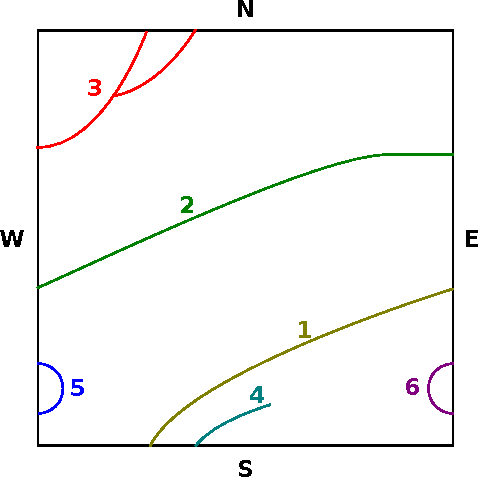
\includegraphics[width=0.75\columnwidth]{fragmentacion/scheme_clusters}
  \caption{Representación esquemática de fragmentos 2D, reconocidos sólo en la celda y no a través de las paredes periódicas, etiquetadas como N, S, W y E.
  Los fragmentos dentro de la celda están etiquetados del 1 al 6.}
\label{fig:scheme_clusters}
\end{figure}

Para hallar las conexiones entre estos fragmentos a través de los contornos, dibujamos un grafo de los fragmentos, donde los conectamos dependiendo de si se conectan o no a través de una pared, y etiquetamos dicha conexión con la etiqueta de la pared.
Por ejemplo, comenzamos con el fragmento 1.
Se conecta con el fragmento 2 a través de la pared E, por lo que agregamos una conexión $1\rightarrow2$ etiquetada como E.
Simétricamente, agragamos una conexión $2\rightarrow1$ etiquetada W.
Ahora vamos por el par 1-3.
Se conecta a través de la pared S, por lo que agregamos $1\rightarrow3$ con la etiqueta S y $3\rightarrow1$ con la etiqueta N.
El fragmento 1 no se conecta con los 4, 5 o 6, por lo que éstas son las únicas conexiones que tenemos para dicho fragmento.
Una vez que hayamos hecho eso, obtenemos el grafo de la figura~\ref{fig:graph_clusters}.

\begin{figure}  \centering
  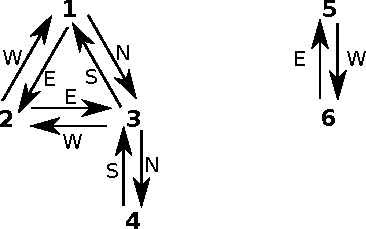
\includegraphics[width=0.45\columnwidth]{fragmentacion/graph_clusters}
  \caption{Grafo de los fragmentos con conexiones etiquetadas por la etiquieta de la pared a través de la cual se conectan.
    El grafo puede ser dividido en dos subgrafos que no se conectan entre ellos: 1--2--3--4 y 5--6.
    Cada uno de estos subgrafos es un fragmento al considerar las condiciones periódicas de contorno.}
\label{fig:graph_clusters}
\end{figure}

Ahora nos preguntamos si estos subgrafos representan un fragmento infinito o no.
Para tener un fragmento infinito necesitamos un ciclo cerrado (lo opuesto no es cierto: tener un circuito cerrado no es suficiente para tener un fragmento infinito, como podemos ver en el subgrafo 5--6), de modo que primero identificamos ciclos y los marcamos como candidatos para fragmentos infinitos.
Cada conexión agrega un ciclo (ya que las conexiones de los fragmentos son ida y vuelta), pero sabemos de inspeccionar la figura~\ref{fig:graph_clusters} que el fragmento 1--2--3 es infinito.
La clave para identificar en los grafos los framentos infinitos es identificar, en el grafo, qué hace al fragmento 1--2--3 infinito.
La característica fundamental del fragmento 1--2--3 es que su ciclo 1--2--3--1 puede ser circulado a través de las paredes E--E--S, mientras que el 5--6 puede ser circulado sólo a través de E--W.
Ahora, para que el fragmento sea infinito, necesitamos que se extienda infinitamente en, al menos, una dirección.
De este modo, una vez que tenemos la lista de paredes del ciclo, creamos una magnitud $I$ asociada a cada ciclo, que se crea de la siguiente manera.
Comenzando con $I=0$, agregamos un valor $M_i$ si hay al menos una pared de tipo $i$.
Los valores son: $M_E= 1$, $M_W = -1$, $M_N = 2$, $M_S = -2$.
Si $I$ no es cero, entonces el ciclo es infinito.
Por ejemplo, el ciclo  E--E--S tiene paredes E y S, de modo que $I = M_E + M_S = -1$ y el ciclo es infinito.
Para el ciclo E--W, $I = M_E + M_W = 0$, y el ciclo es finito.

\section{Expansión}\label{sc:expansion}
Para expandir la materia rica en neutrones que simula un sistema infinito con condiciones periódicas de contorno, seguimos el método del \emph{big bang microscópico}, explicado por Holian y Grady en Ref.~\cite{holian_fragmentation_1988} y usado por la expansión de sistemas infinitos previamente~\cite{dorso_onset_1996}.
Consiste en una expansión de la celda de simulación a un ritmo isotrópico y constante $\dot{\eta}$:
\begin{equation}
  L(t) = L_0\,(1+\dot{\eta}\,t)
\end{equation}
donde $L$ es la longitud inicial de la celda de simulación en cada dirección y $L_0$ es la longitud inicial.
Sólo con esta modificación del tamaño de la caja, el sistema se expandiría dinámicamente.
Para simular una expansión, necesitamos también que las partículas tengan una velocidad radial extra que concuerde con la de la celda en los bordes de la simulación:
\begin{equation}
  \mathbf{v} = \mathbf{v_0} + \dot{\eta}\,\mathbf{r_0}
\end{equation}

Ya que estamos trabajando con condiciones periódicas de contorno, cuando una partícula cruza un contorno, debemos considerar la expansión original, por lo que no cambiamos sólo la posición de la partícula sino también la velocidad.
Por ejemplo, si la partícula cruza el contorno izquierdo de la caja periódica, la velocidad de la partícula imagen $v_i^\dagger$ en el lado derecho debe ser modificada $v_i^\dagger = v_i + L_0\,\dot{\eta}$.
Esta prescripción para la expansión es matemáticamente equivalente a la ley de Hubble en astrofísica~\cite{chikazumi_quantum_2001}.
Es interesante notar que la expansión con esta prescripción es (para el sistema infinito simulado) adiabática: del momento inicial en adelante, no se agrega más energía al sistema.

\section{Fragmento infinito}
En la figura~\ref{fig:morpho} mostramos los estados inicial y final de la expansión de la celda principial de $N=11000$ partículas para velocidades de expansión muy bajas.
Podemos ver que, más allá de que la configuración inicial muestra una distribución de partículas compacta, la configuración final consiste de \emph{gnocchi} (casi esféricos) con una masa de alrededor de 80 partículas.

\begin{figure} \centering
  \begin{subfigure}[h!]{0.45\columnwidth}
    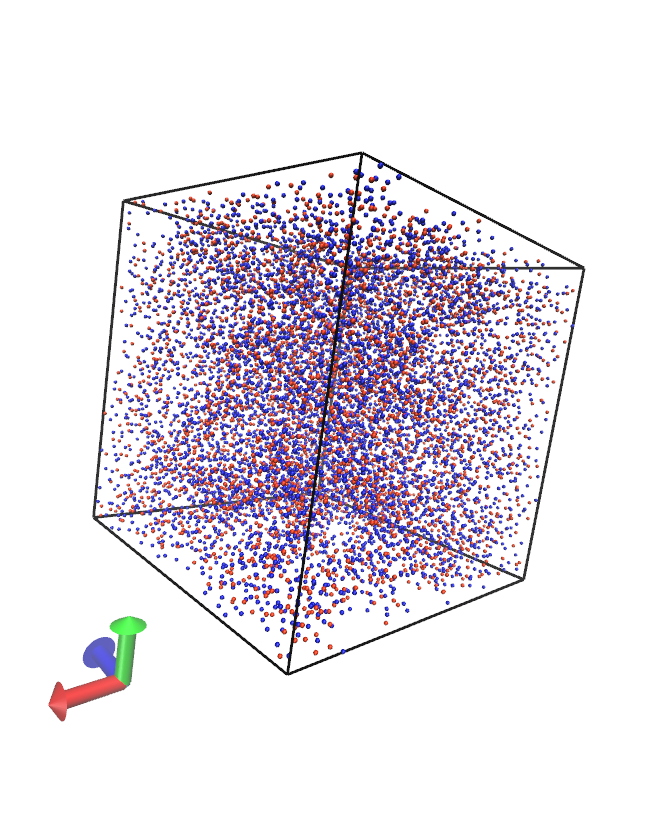
\includegraphics[width=\columnwidth]{fragmentacion/initial}
    \caption{$\eta = 0.0001\,\text{fm/c}$}
    \label{subfig:initial}
  \end{subfigure}
  \begin{subfigure}[h!]{0.45\columnwidth}
    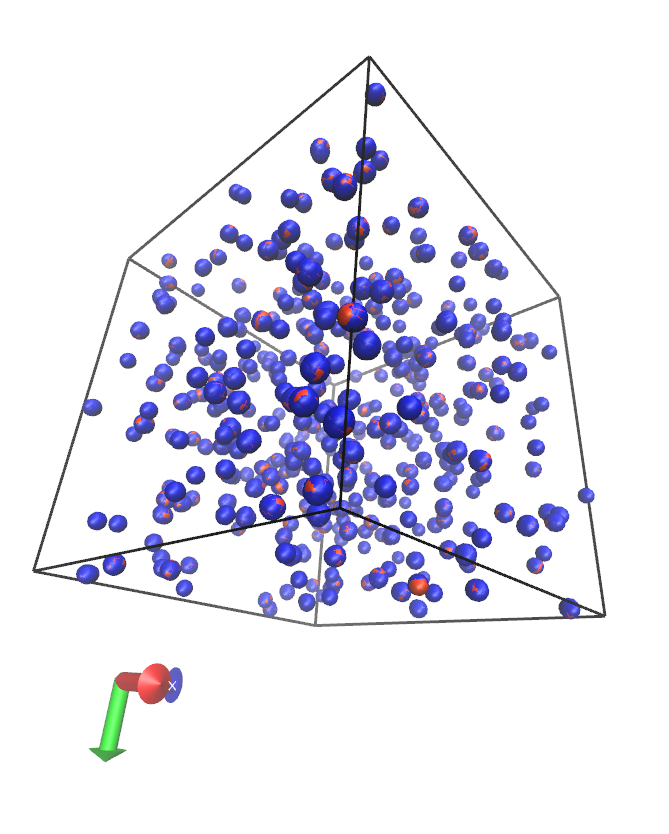
\includegraphics[width=\columnwidth]{fragmentacion/expanded}
    \caption{$\eta = 0.0005\,\text{fm/c}$}
    \label{subfig:expanded}
  \end{subfigure}
  \caption{Estructuras de un sistema en su configuración inicial~\ref{subfig:initial} y el sistema expandido final~\ref{subfig:expanded}.
    En el sistema expandido podemos ver que se forman fragmentos de tipo \emph{gnocchi}.}
  \label{fig:morpho}
\end{figure}

En la figura~\ref{fig:infinite} mostramos la fracción de partículas en la celda principal que forman parte de un cluster infinito (\emph{Fracción de Fragmento Infinito}, FFI).
Podemos ver fácilmente que en las primeras etapas de la evolución, como la temperatura es baja, la mayor parte del sistema en la celda principal pertenence al fragmento infinito.
Sin embargo, a medida que evoluciona el sistema de acuerdo a la velocidad de expansión, la FFI disminuye y llega a cero rápidamente, implicando que no hay fragmentos infinitos en el sistema.

\begin{figure}
  \centering
  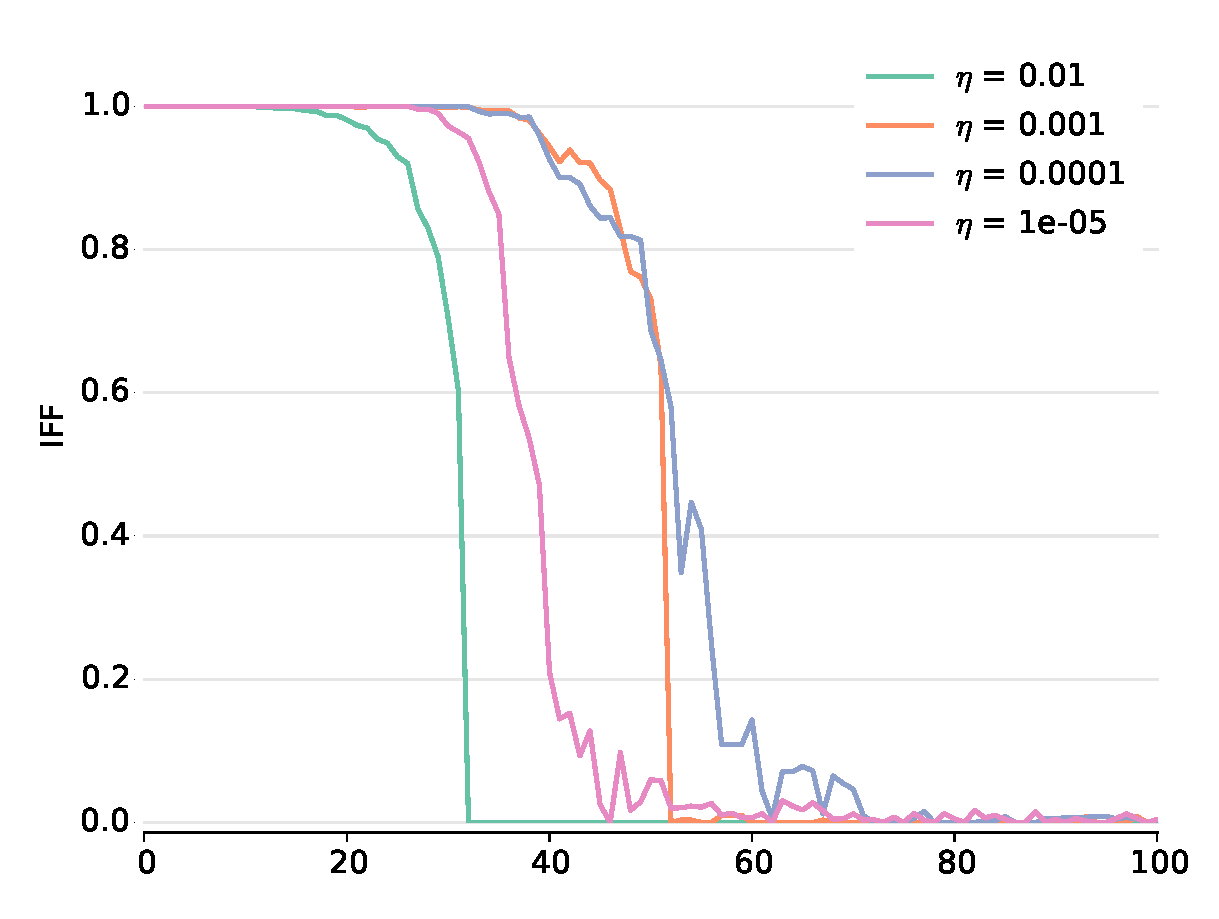
\includegraphics[width=0.75\columnwidth]{fragmentacion/infinite.pdf}
  \caption{Fracción de Fragmento Infinito (ver texto) en función de la longitud de la celda principal.
    Para todas las velocidades de expansión mostradas el FFI va a cero en el régimen asintótico.}
  \label{fig:infinite}
\end{figure}

\section{Fragmentos asintóticos}

La figura~\ref{fig:distribution} muestra la distribución de fragmentos asintóticos para cuatro distintas velocidades de expansión.
En este caso, el algoritmo MSTE fue aplicado sobre la celda principal, considerando las condiciones periódicas de contorno y sabiendo que no hay fragmento infinito, como se ve de la figura~\ref{fig:infinite}.
Podemos ver que a medida que aumenta la velocidad de expansión, la distribución de fragmentos muestra la típica transición de U-shaped a decaimiento exponencial.
Entre estas dos, aparece una distribución de tipo ley de potencias.
En particular, la figura~\ref{subfig:9e-3} muestra que con una expansión de $\eta = 0.009\,\text{fm/c}$ obtenemos una ley de potencias.
Es interesante notar que a diferencia de casos típicos de estudios de fragmentos, como percolación o sistemas de Lennard-Jones, debido a la presencia del término de repulsión de Coulomb, no es posible ver un fragmento infinito en el régimen asintótico.

\begin{figure} \centering
  \begin{subfigure}[h!]{0.45\columnwidth}
    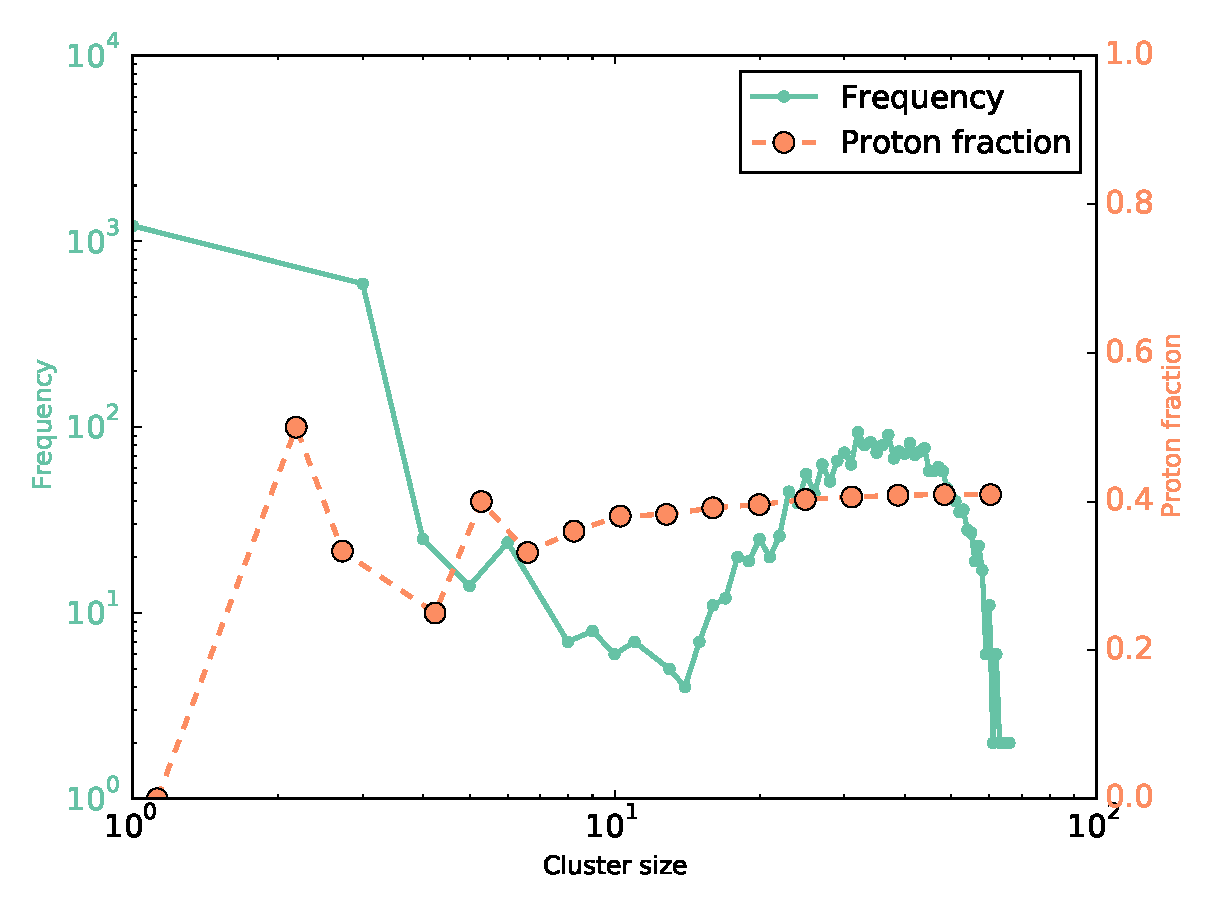
\includegraphics[width=\columnwidth]{fragmentacion/cluster_1e-4}
    \caption{$\eta = 0.0001\,\text{fm/c}$}
    \label{subfig:1e-4}
  \end{subfigure}
  \begin{subfigure}[h!]{0.45\columnwidth}
    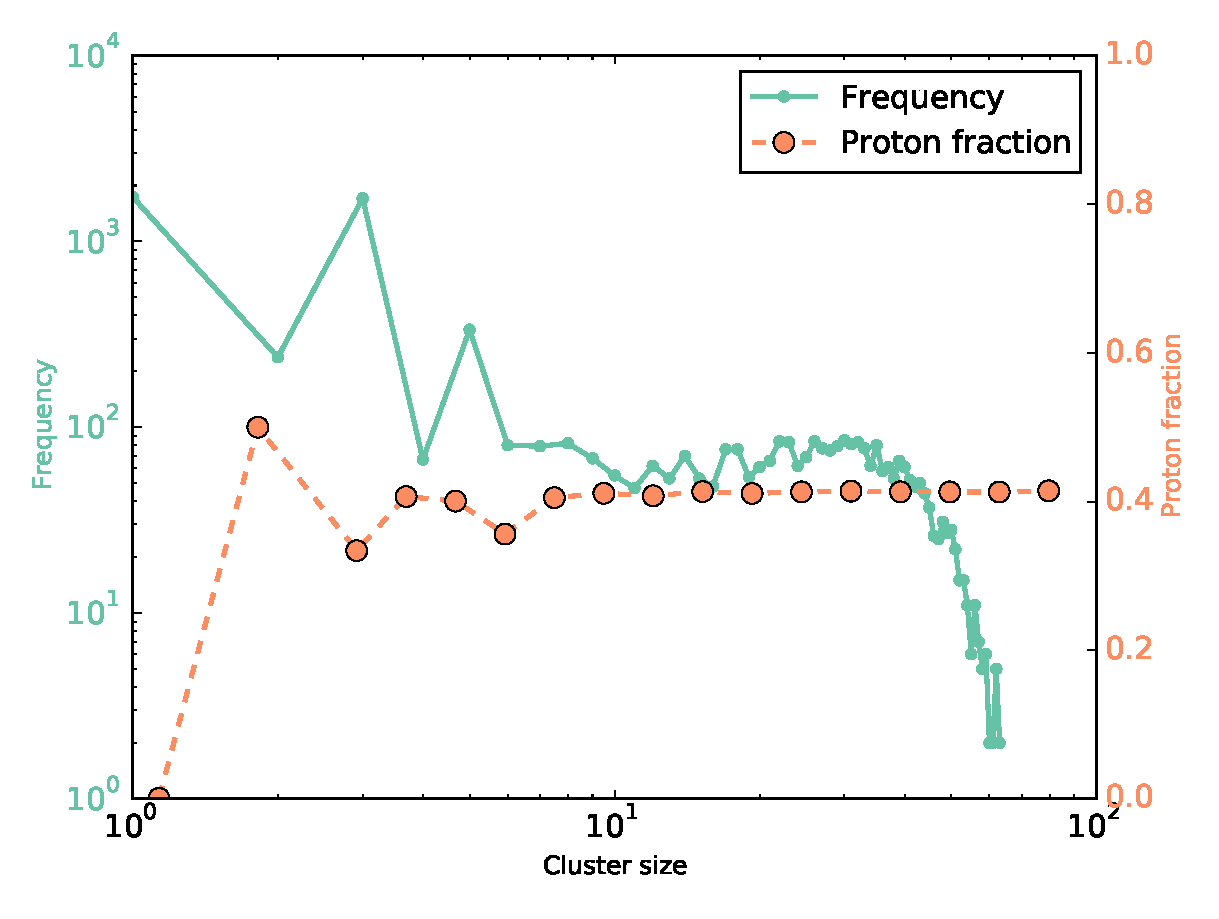
\includegraphics[width=\columnwidth]{fragmentacion/cluster_5e-4}
    \caption{$\eta = 0.0005\,\text{fm/c}$}
    \label{subfig:5e-4}
  \end{subfigure}
  \begin{subfigure}[h!]{0.45\columnwidth}
    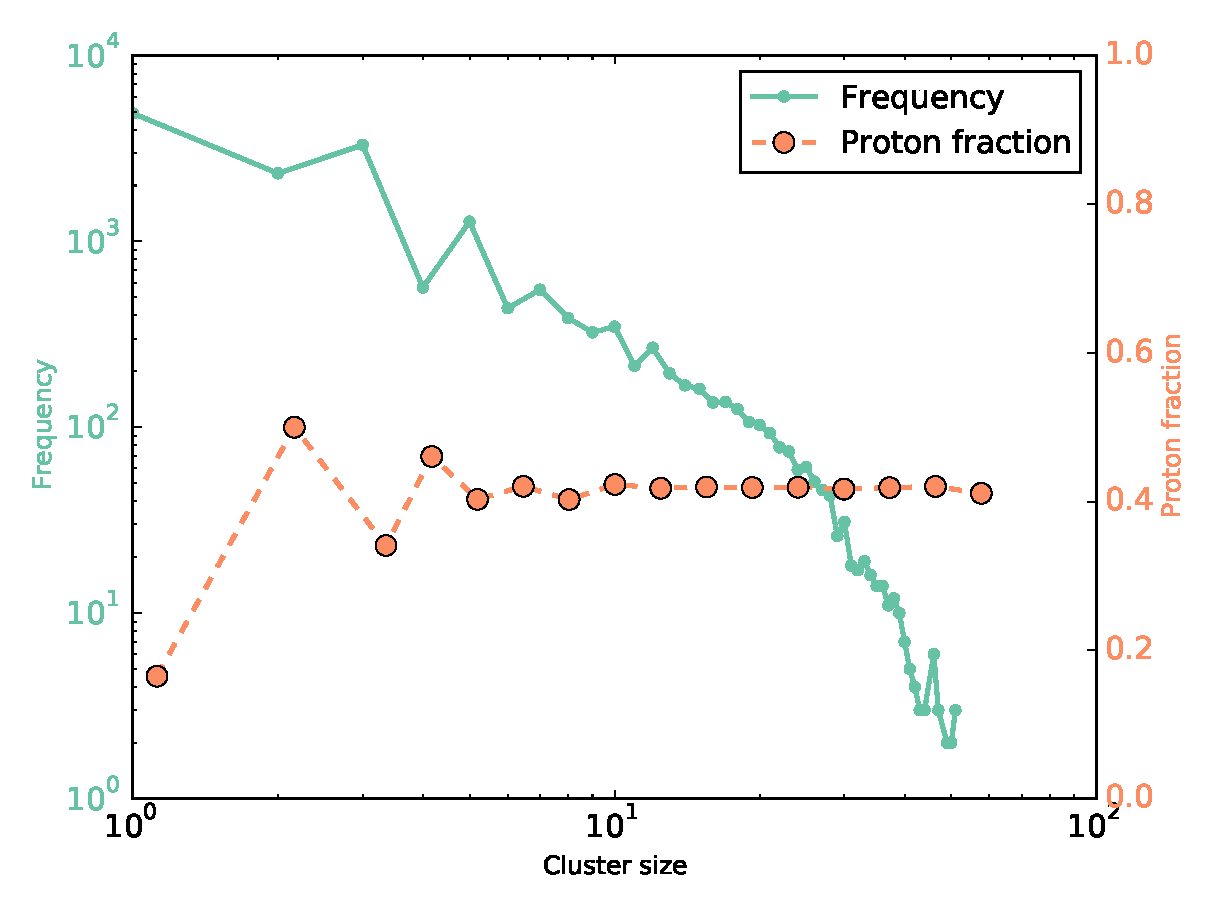
\includegraphics[width=\columnwidth]{fragmentacion/cluster_9e-3}
    \caption{$\eta = 0.009\,\text{fm/c}$}
    \label{subfig:9e-3}
  \end{subfigure}
  \begin{subfigure}[h!]{0.45\columnwidth}
    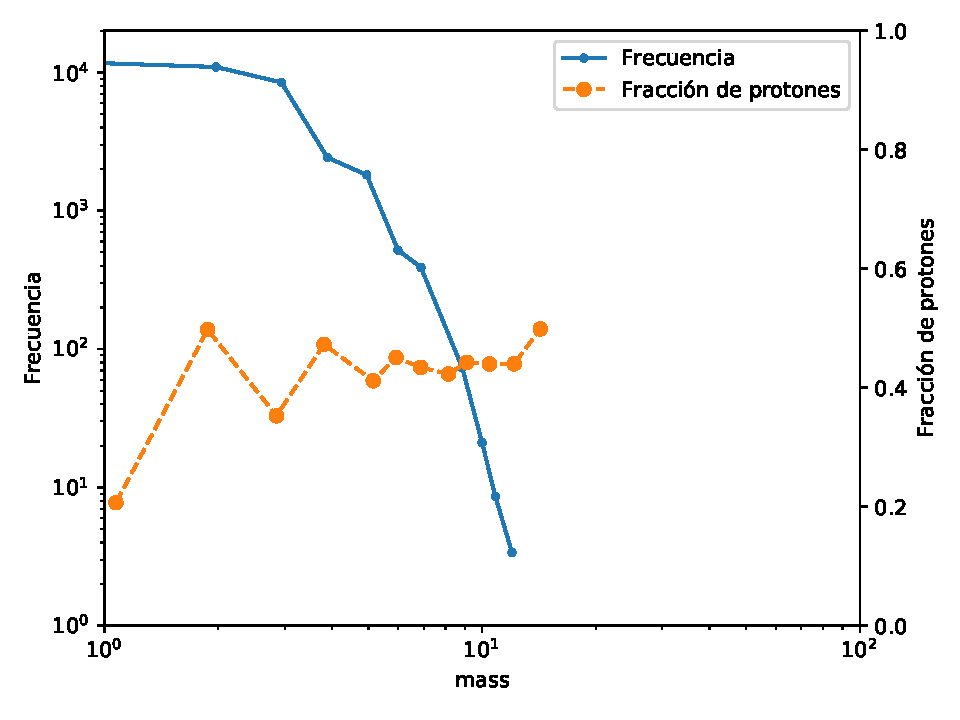
\includegraphics[width=\columnwidth]{fragmentacion/cluster_3e-2}
    \caption{$\eta = 0.03\,\text{fm/c}$}
    \label{subfig:3e-2}
  \end{subfigure}
  \caption{Distribución de masa de fragmentos.
    Las etiquetas aumentan junto a la velocidad de expansión.
    El sistema consiste de 11000 partículas con $x=0.4$ y densidad inicial $\rho_0 = 0.08\,\text{fm}^{-3}$}
  \label{fig:distribution}
\end{figure}

\section{Conclusiones}

Desarrollamos experimentos numéricos de sistemas expandidos homogéneamente  y, para analizar la estructura del sistema en función del tiempo, desarrollamos una herramienta basada en análisis de grafos para identificar fragmentos infinitos para cualquier tipo de fragmentos aditivios.
Una vez que esta formalismo fue aplicado a las simulaciones mencionadas, pudimos identificar la región en la que se da una distribución de fragmentos de tipo ley de potencias.
Esta distribución tiene formas desde U-shaped hasta decaimiento exponencial.
